\section{Lezione 16} \hfill 08/04/2026\\
Da piccolo ha un legno piuttosto elastico, in modo da poter resistere ai movimenti della neve (es. scivolamento, reptazione); per questo motivo da adulta può assumere una particolare forma sciabolata alla base.\\
Rispetto alla protezione da valanghe, è abbastanza inefficiente, in quanto che in inverno non ha chioma.\\
Il legno del larice è:
\begin{itemize}[nosep]
    \item molto duro;
    \item differenziato in alburno e durame (rosso, con anelli molto netti);
    \item molto durabile: buono per usi esterni;
    \item pesante (definito perciò ``hardwood'');
    \item è molto stabile (si muove poco): usato per pavimenti, travi, mobili, infissi.
\end{itemize}
È stato molto apprezzato dalla Repubblica di Venezia, sia per la costruzione degli alberi delle navi e sia per le fondamenta della Città.\\
I lariceti sono più abbondanti sulle Alpi occidentali rispetto alle orientali (es. Cortina, Alto Adige). Infatti, in questa area è stata più forte la mano antropica (es. miniere, guerre).\\
Dove ci sono lariceti, molto spesso sono stati favoriti dall'uomo, che li ha mantenuti tali (impedendo l'evoluzione):
\begin{itemize}[nosep]
    \item il legno è molto pregiato;
    \item la chioma è leggera verde-chiara, che permette lo sviluppo di una coltre erbacea sotto di essa (sistema di lariceti-pascolati).
\end{itemize}
L'unico trattamento che permette la rinnovazione del larice è il taglio raso (almeno 3000-5000 \unit{m^2}): in Italia però è vietato. Inoltre, ci sarebbe un doppio problema:
\begin{itemize}[nosep]
    \item nascita di una coltre erbacea;
    \item gli aghi a terra fanno fatica a mineralizzare (marcire), creando uno strato denso di foglie e bloccando la rinnovazione.
\end{itemize}
Un ambiente colonizzato dal larice non favorisce la propria rinnovazione: il suo destino è quello di andare verso un altro popolamento.\\
L'unico modo per risolvere il problema è quello di scarificare (rompere il tappeto di aghi), portando alla luce il suolo minerale. Questa cosa non può essere fatta in modo andante, perché creerebbe dissesti. Conviene perciò scarificare piccole aree, a scacchiera e di 3-10 mq, in modo che non ci sia soluzione di continuità.\\
Il lariceto è destinato a diventare qualcos'altro, lasciando spazio alle definitive:
\begin{itemize}[nosep]
    \item a quote basse tendenzialmente una pecceta (es. quello che sta succedendo a Cortina);
    \item a quote elevate tendenzialmente il pino cembro (specie leader del piano subalpino).
\end{itemize}
\begin{figure}[htbp]
     \centering
     % Prima Immagine
     \begin{subfigure}[b]{0.33\textwidth}
         \centering
         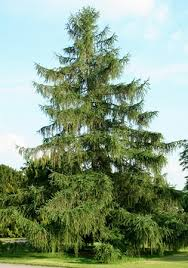
\includegraphics[width=\textwidth]{immagini/larice_portamento.jpg}
        %\caption{}
     \end{subfigure}
     \hfill % Spazio elastico tra le immagini
     % Seconda Immagine
     \begin{subfigure}[b]{0.3\textwidth}
         \centering
         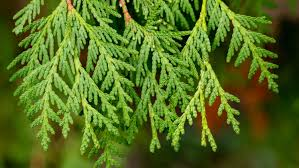
\includegraphics[width=\textwidth]{immagini/larice_foglie.jpg}
        %\caption{}
     \end{subfigure}
     \hfill % Spazio elastico tra le immagini
     % Terza Immagine
     \begin{subfigure}[b]{0.33\textwidth}
         \centering
         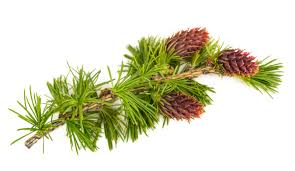
\includegraphics[width=\textwidth]{immagini/larice_coni.jpg}
        %\caption{}
     \end{subfigure}
    \caption{Larice}
     \label{fig:larice}
\end{figure}
\subsection{Pino cembro - Pinus cembra}
Viene anche detto cirmolo o cembro.\\
Questa specie è:
\begin{itemize}[nosep]
    \item la leader del piano subalpino;
    \item come tutti i pini è fortemente eliofilo;
    \item con un apparato radicale fittonante particolare, con serie di radici che entrano nel terreno in modo verticale, orizzontale e diagonale (es. regola della mano destra);
    \item l'unico pino indigeno europeo a 5 aghi;
    \item un relitto delle glaciazioni (arrivato dalla Siberia fino all'Europa occidentale);
    \item con un areale tendenzialmente più occidentale che orientale nelle Alpi (ad est non si spinge oltre al Cadore);
    \item capace di crescere sulle rocce
\end{itemize}
Il pino cembro ha un seme pesante (come il pino domestico), e matura i coni in 3 anni (producendo pinoli). Questo fa si che la disseminazione sia zoocora, a carico della nocciolaia, che prende i pinoli con il becco e ne fa dei piccoli depositi, da poterne mangiare in inverno. I mucchietti vengono fatti dove la neve fonde prima, o dove proprio non arriva: in questo modo avviene la nascita di pini a mucchietti.\\
Laccrescimento è estremamente lento, mettendoci fino a 100 anni per uscire dalla coltre nevosa: in questo periodo può essere attaccato dalle muffe presenti nelle nevi.\\
Quando la pianta esce dalla neve, la crescita è costante, anche se la velocità non è eccessiva.\\
Il posto ideale dove si sviluppa è a partire dal lariceto (es. dove c'è la coltre di neve rotta, è presente la nocciolaia). Molto spesso i cembri nascono sulle rocce o alla base di vecchi larici.\\
In questo modo c'è la formazione dei larici-cembreti (che tendenzialmente diventeranno delle cembrete pure).\\
Il cembro tende a formare collettivi (come tutte le specie del piano subalpino), che vanno gestiti singolarmente (es. ``o si tiene tutto il collettivo o si toglie tutto il collettivo'').\\
Il pino cembro è importante dal punto di vista protettivo (avendo la chioma scura, pesante e densa, riduce la formazione delle valanghe), e produttivo (il legno è molto morbido, profumato, usato per mobili e da intaglio).\\
Non si fa selvicoltura con il cembro; eventualmente si può estrarre dal bosco solamente gli individui danneggiati da disturbi naturali (e comunque lavorando sempre su tutto il collettivo).\\
In un larice-cembreto conviene favorire il pino cembro, che è la specie definitiva.
\subsection{Limite del bosco}
Tendenzialmente il bosco non può salire sopra la isoterma dei 10 gradi del mese di luglio (linea che unisce la temperatura media dell'aria nel mese di luglio).\\
Il limite del bosco è determinato da:
\begin{itemize}[nosep]
    \item temperatura;
    \item suolo o non suolo;
    \item esposizione (a sud più alto, mentre a nord più basso);
    \item definizione su cosa si considera bosco in quota (es. ecologia, giurisprudenza). 
\end{itemize}
Esistono più limiti del bosco, a seconda di cosa si vuole intendere, dal basso verso l'alto:
\begin{itemize}[nosep]
    \item limite del bosco commerciale (timber-line): linea per il quale può essere utilizzato commercialmente. Tendenzialmente è il limite del bosco chiuso;
    \item limite del bosco con una idea ecologica (a collettivi);
    \item limite degli alberi (sottoforma di albero);
    \item limite del krummholz (``legno contorto''), limite degli alberi sottoforma di arbusti. 
\end{itemize}
Attualmente, il limite del bosco sta diventando importante per via dei cambiamenti climatici, poiché tendenzialmente si sta alzando. Il limite del bosco non commerciale in passato era a 2000-2200 m s.l.m. sulle Alpi orientali e 2200-2300 m s.l.m. sulle Alpi occidentali; negli ultimi 50 anni, questo limite si è alzato di 100-200 metri.\\
Non è detto che si rendano disponibili nuove aree forestali, perché potrebbe non esserci suolo (es. scivolamento della neve o roccia viva) o perché ci potrebbero essere eccessivi disturbi.\\
Tutti questi popolamenti ad elevate quote svolgono la funzione di protezione, turismo e ricreatività.\\
Ad elevate quote, tutti i processi rallentano, causa maggiormente le ridotte temperature.\\\\
%\subsection{Rinnovazione naturale}
\fbox{ \centering
    \begin{minipage}{0.95\textwidth} 
La rinnovazione naturale è la migliore, perché è quella più giusta. 
    \end{minipage}}
\subsection{Arboricoltura da legno}
Il pioppo è la specie fondamentale dell'arboricoltura da legno italiana.\\
I pioppi italiani sono il:
\begin{itemize}[nosep]
    \item bianco: le facce inferiori delle foglie sono pubescenti, è il pioppo meno legato all'acqua;
    \item nero: fortemente legato all'acqua (boschi ripariali), non sopporta di avere le radici in acqua ma ne vuole in continuità (perché la crescita è elevata);
    \item tremulo: è un pioppo montano, legato alla presenza di acqua (non quanto l'ontano, ma quasi);
    \item ibrido (tra il tremulo ed il bianco).
\end{itemize}
In arboricoltura i pioppi hanno una discreta capacità pollonifera caulinare, che nelle vecchie piante non esiste e che dopo 2-3 ceduazioni scompare. Ogni tanto il pioppo tremulo produce polloni radicali, creando così un individuo a ceduo.\\
In arboricoltura il pioppo tremulo non viene utilizzato, perché non è possibile moltiplicarlo per talea (ma solo per seme): sarebbe una specie ottima perché ha molti gli aspetti positivi per la produzione (fusti regolari e cilindrici, corteccia sottile).\\
In arboricoltura viene utilizzato molto il pioppo ibrido, incrocio tra il nero americano (Populus deltoides) e ed il nero europeo (Populus nigra): commercialmente vengono chiamati canadesi. I cloni delle specie solamente americane sono chiamati ``caroliniani''.\\
Il pioppo è una specie con individui maschi e femmina (i cloni ottenuti possono essere perciò maschi o femmine).\\
La pioppicoltura venne inventata in Italia, fatta con i pioppi e successivamente con i loro cloni ibridi.\\
I cloni più produttivi della prima generazione erano molto soggetti alla defogliazione primaverile (Venturia pupulina). La seconda generazione, resistente alla defogliazione era soggetta al un fungo che imbruniva le foglie. La terza generazione era soggetta alla batteriosi. Al quarto ciclo, sono nati i cloni MSA (Maggiore Sostenibilità Ambientale).\\
Il pioppo viene commercializzato a quintali, e non a metri cubi (le densità, in funzione all'umidità, sono diverse): per questo motivo sono stati privilegiati i cloni più leggeri.\\
Oggi i pioppi vengono coltivati per creare sfogliati o compensati. Per standardizzare il processo di creazione di sfogliati, viene preferito il clone I214.\\
La coltivazione di un clone rende la produzione uguale: in questo modo vengono riprodotti gli stessi pregi e gli stessi difetti. La soluzione sarebbe quella di creare impianti polispecifici o policlonali: non verrebbero più commercializzati.\\
In pioppicoltura si utilizzano le talee (ovvero una porzione di fusto o di ramo), lunghe circa 20 cm e di diametro 2-3 cm, possibilmente avente 3 gemme; è in grado di germinare e ricostruire un identico individuo, come quello di partenza della talea. Non si usano parti apicali per creare la talea, soprattutto del pioppo, perché non sono ben lignificate e perché non riescono a riprodursi.\\
Una talea piantata che produce un fusto ed un apparato radicale avventizio, viene chiamata barbatella. In pioppicoltura la barbatella viene chiamata pioppella, e solitamente viene commercializzata senza rami (può avere o meno le radici). Se non ha le radici viene chiamata ``astone".\\
Le pioppelle vengono commercializzate di 1-2 anni: se di 1 anno sono alte 3-4 metri e con diametri di 2-4 \unit{cm}, mentre se di 2 anni sono alte 6-8 metri e hanno diametri di 4-8 \unit{cm}.\\
In genere, è meglio una pioppella di un anno, perché costa meno e produce più tronco.